\chapter[Análise e Projeto do Sistema]{Análise e Projeto do Sistema}

Este capítulo apresenta a análise e projeto do sistema de acordo com os requisitos levantados, a figura 3 apresenta uma visualização da arquitetura planejada, demonstrando como seus módulos e atores interagem.

\begin{figure}[htp]
    \centering
    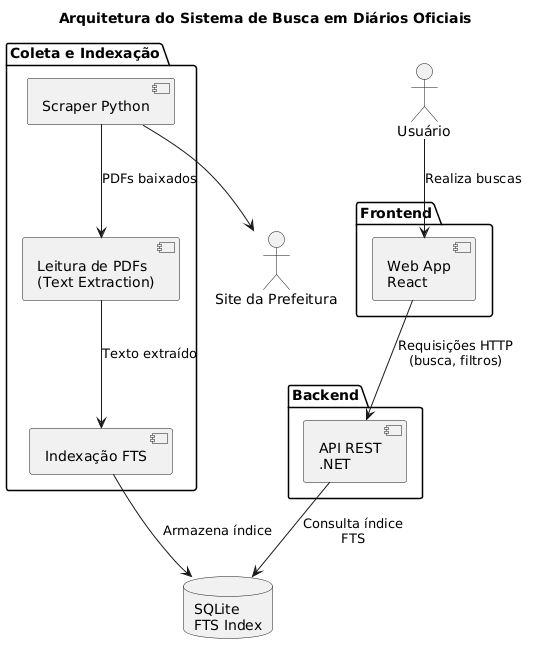
\includegraphics[width=0.7\linewidth]{figs/RPBFRjD.png}
    \caption{Arquitetura do Sistema de Recuperação}
    \label{fig:placeholder}
\end{figure}

%<Este capítulo tem como objetivo analisar e projetar a solução do sistema de acordo com os requisitos levantados e validados no capítulo 2. Para isso, deve-se ter uma visão geral da arquitetura do sistema e a modelagem da solução do sistema através de diagramas.>

\section{Modelo de Domínio do Sistema}

O modelo inicial de domínio da figura 6 representa o problema que o sistema buscar resolver, demonstrando o fluxo conceitual: uma cidade publica vários diários que são compostos por várias páginas, as páginas são indexadas em um índice textual que é consultado conforme os critérios de busca do usuário para que os documentos sejam recuperados e exibidos de acordo com estes critérios.

\begin{figure}[htp]
    \centering
    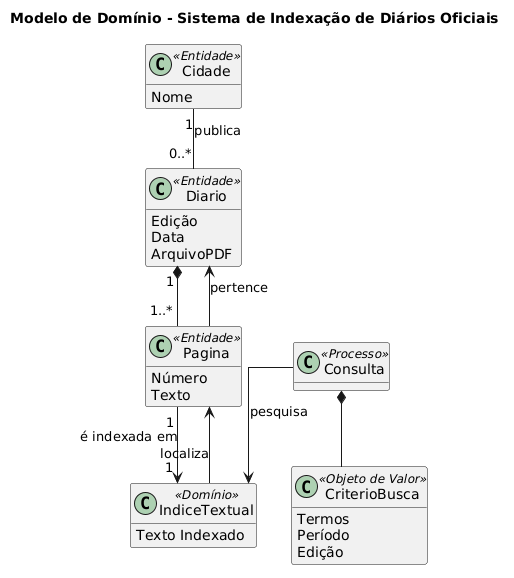
\includegraphics[width=0.7\linewidth]{figs/diagramas/ModeloDominioDoSistema.png}
    \caption{Modelo de domínio do sistema}
    \label{fig:placeholder}
\end{figure}

A partir deste modelo já é possível ter uma ideia inicial dos módulos que compõem o sistema. Se faz necessário um componente de obtenção e indexação dos documentos, um componente responsável pelas consultas e um componente de exibição dos resultados, no caso deste trabalho, como foi mostrado na figura 5, o paralelo são os módulos de coleta e indexação, backend e frontend, respectivamente.
%<Neste item deve ser apresentado o modelo do domínio, que representa um primeiro modelo conceitual do diagrama de classes. Posteriormente, esse diagrama deve ser validado e complementado para compor o diagrama de classes final.>

%\begin{figure}[h]
%    \centering
%	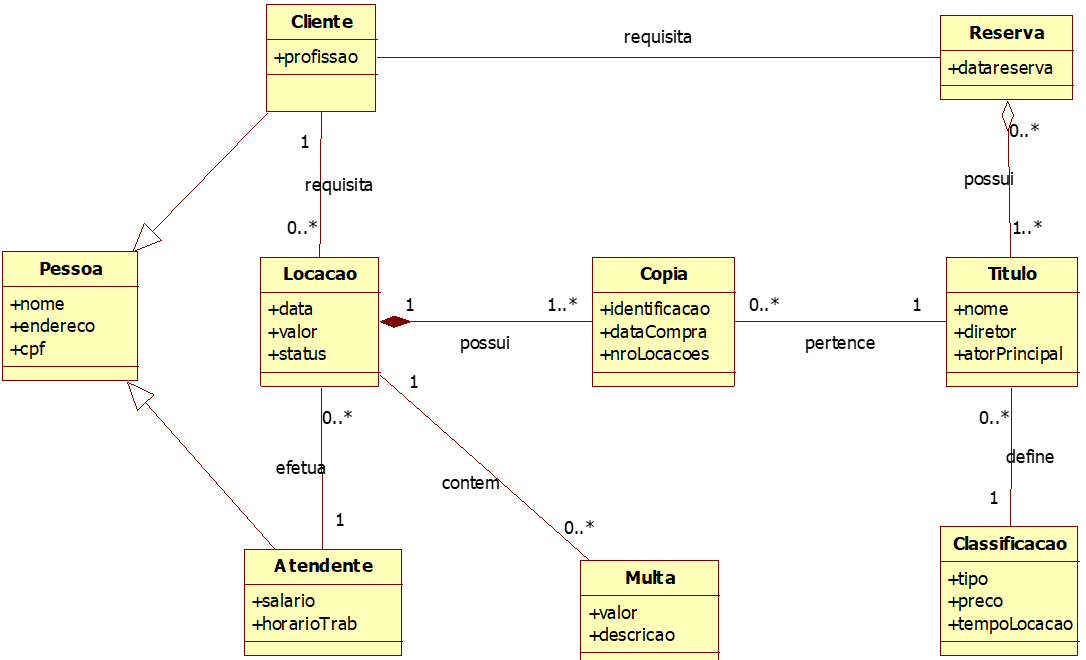
\includegraphics[width=1.0\linewidth]{figs/Modelo_conceitual.png}	\caption[Exemplo de Modelo Conceitual do Sistema.]{Exemplo de Modelo Conceitual do Sistema.}
%	\label{fig:ModeloConceitual}
%\end{figure}
\section{Diagramas de Sequência do Sistema}
%<Neste item devem ser apresentados os diagramas de seqüência essenciais (mais importates) ao sistema. Um diagrama de seqüência representa interações de objetos organizadas em uma seqüência temporal, apresentando os objetos que participam da interação e a seqüência das mensagens trocadas. O diagrama de seqüência deve validar o diagrama de classes e vice-versa. Pode ser usado como alternativa ao diagrama ed sequência o diagrama de colaboração.>
A seguir são apresentados os diagramas de sequência mais relevantes do sistema. A figura X apresenta o diagrama criado inicialmente para representar a sequência da busca textual, partindo da interação do usuário com o frontend enviando uma requisição de busca nos diários indexados e retorno da resposta pela API.

\begin{figure}[htp]
    \centering
    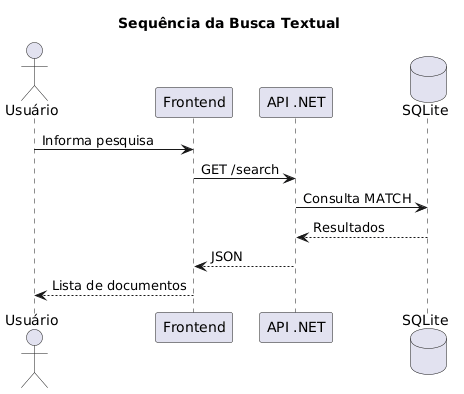
\includegraphics[width=0.5\linewidth]{figs//diagramas/DiagramaDeSequenciaDeBusca.png}
    \caption{Diagrama de sequência da busca}
    \label{fig:placeholder}
\end{figure}

Nos itens seguintes são apresentados os diagramas  referentes ao processo de coleta e indexação, processo de busca e processo de visualização dos documentos, assim como os requisitos funcionais correspondentes a estes processos.

%\subsection{Diagramas de Sequência - RF001 - Nome do Requisto Funcional}
%\begin{figure}[h]
%    \centering
%	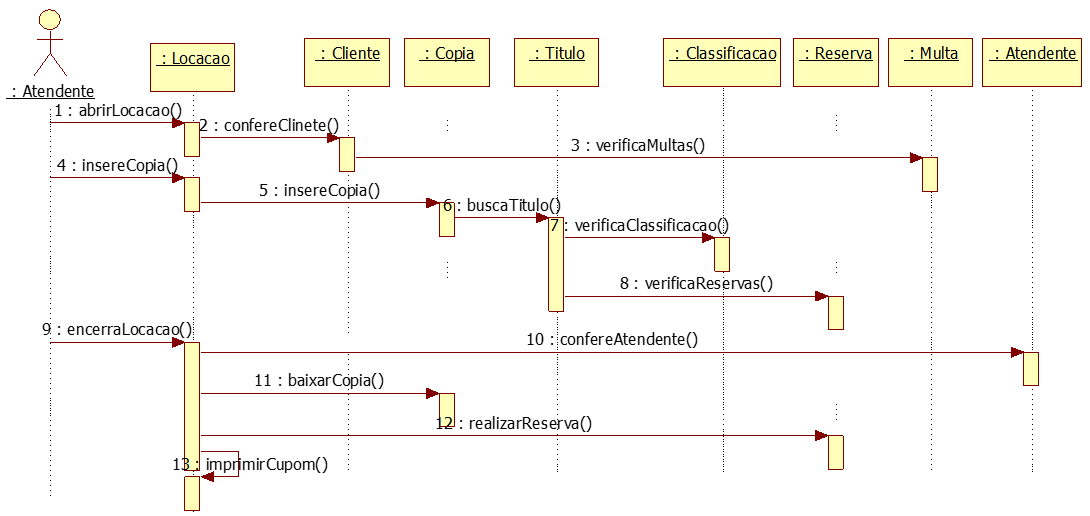
\includegraphics[width=1.0\linewidth]{figs/Sequencia.png}
%	\caption[Exemplo de Diagrama de Sequência - RF001.]{Exemplo de Diagrama de Sequência - RF001.}
%	\label{fig:DiagramaSequencia}
%\end{figure}

\subsection{Diagramas de Sequência - (RF001, RF002, RF003, RF004) - Processo de Coleta e Indexação}

O diagrama do processo de coleta e indexação abrange os requisitos funcionais RF001, RF002, RF003 e RF004, nele é descrito o processo realizado para coleta e indexação dos documentos, sendo um operador manual ou ferramenta de agendamento de execução que inicia o processo de execução da ferramenta, que cuida da obtenção da lista de documentos, download e indexação no banco SQLite.

\begin{figure}[htp]
    \centering
    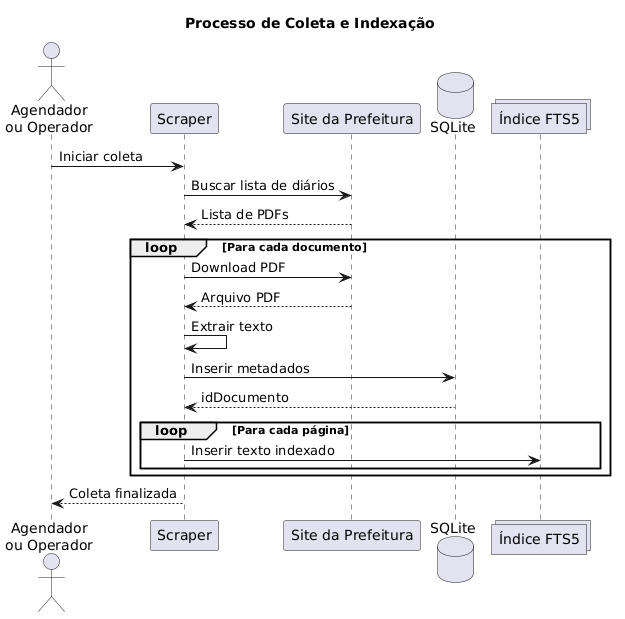
\includegraphics[width=0.6\linewidth]{figs//diagramas/SeqColetaEIndex.png}
    \caption{Processo de Coleta e Indexação}
    \label{fig:placeholder}
\end{figure}

A indexação é feita a partir da leitura de cada página do documento separadamente, que salva na tabela "docs\_fts" o número de página, conteúdo e id de documento correspondente. Após a indexação total das páginas do documento o processo é concluído.

\subsection{Diagramas de Sequência - (RF005, RF006, RF007) - Processo de Busca}

Já o diagrama de busca abrange os requisitos funcionais RF005, RF006 e RF007, nele é descrito o processo de busca desde a requisição feita pelo usuário no frontend web, passando pelos módulos de backend até o retorno da lista de documentos obtidos de acordo com a pesquisa realizada. Neste processo o usuário define termos de busca, filtragem por datas e edição e a partir disto a API REST monta a consulta que será realizada ao banco de dados.

\begin{figure}[htp]
    \centering
    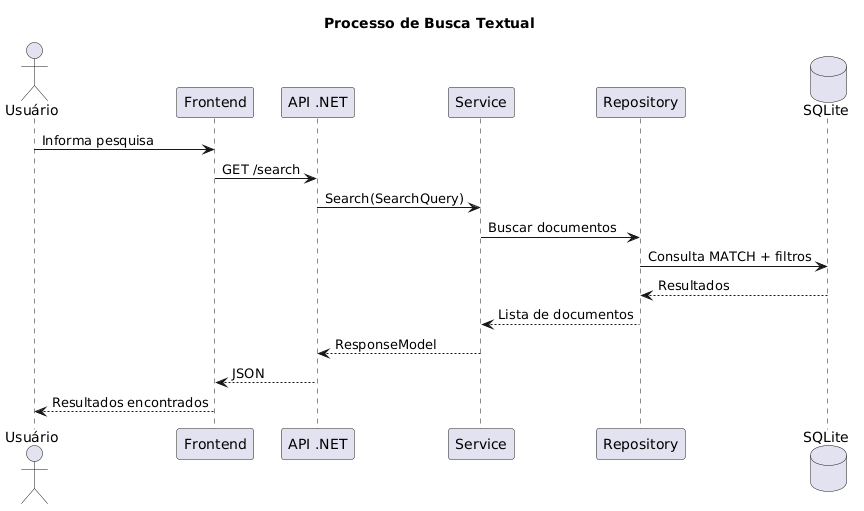
\includegraphics[width=0.8\linewidth]{figs//diagramas/SeqBuscaTextual.png}
    \caption{Processo de Busca}
    \label{fig:placeholder}
\end{figure}

 A API possui um endpoint de pesquisa ("/search"), que recebe a requisição com os dados de busca definidos pelo usuário e a montagem da consulta é feita a depender de quais dados de busca foram enviados, sendo possível buscar apenas por consulta de texto, datas e edição, ou o conjunto destas informações. O resultado da consulta realizada é serializado em formato JSON e devolvido ao front para listagem.

\subsection{Diagramas de Sequência - (RF008, RF009, RF010) - Visualização do Documento}

O diagrama de visualização da figura X expande o diagrama do processo de busca da figura X, fornecendo uma visão de como é estruturada a busca pelos documentos que o usuário pretende visualizar.

\begin{figure}[htp]
    \centering
    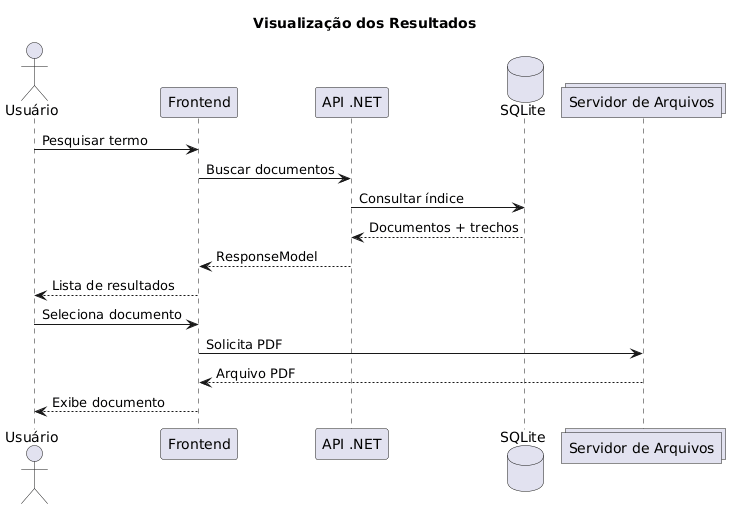
\includegraphics[width=0.8\linewidth]{figs//diagramas/SeqVisualizacaoDosResultados.png}
    \caption{Visualizacao dos Resultados}
    \label{fig:placeholder}
\end{figure}

Depois que o usuário definiu quais termos de busca e filtros serão aplicados, esta informação é repassada para a API que realiza a busca na base de dados usando a consulta definida. Primeiramente é obtida a lista de id's de documentos que resultam da busca realizada, a partir destes id's são obtidos os metadados e as 3 primeiras páginas de cada um destes documentos que contém os trechos pesquisados (no caso de busca textual), caso a busca seja feita somente por data a API retorna somente a primeira página do documento. O frontend recebe a resposta da consulta com estes dados e faz a listagem usando as informações de edição, data e link de acesso ao pdf, além de utilizar as páginas que contém os trechos pesquisados para exibir a prévia na listagem.

\section{Modelagem de Dados do Sistema}
\subsection{Modelo Lógico de Dados do Sistema}

A figura XX apresenta o modelo de Entidade-Relacionamento construído nas versões iniciais do desenvolvimento e o modelo final após o desenvolvimento do sistema. Como o SQLite não possui um tipo de dado específico para armazenar datas, apenas funções de tempo que realizam operações usando tipos numéricos e de texto, a ideia inicial foi armazenar os valores de ano, mês e dia de forma separada em campos com tipos de dados numéricos.

\begin{figure} [htp]
    \centering
    \includegraphics[width=0.7\linewidth]{figs//diagramas/DERjunto.png}
    \caption{Modelo Entidade Relacionamento}
    \label{fig:placeholder}
\end{figure}

Com o avanço do desenvolvimento, este modelo foi alterado para que estes valores fossem armazenados em um único campo de texto, utilizando o formato YYYY-MM-DD \cite{iso8601} para representar a data, o que permite que a tabela fique mais simplificada e as consultas que dependem de filtragem por tempo também sejam melhoradas. Além disso, o formato armazenado é reconhecido por diferentes linguagens de programação que possuem funções que trabalham com datas, como por exemplo C\# usado na API backend que possui as classes "DateTime" e "DateOnly". O campo "indexado" também foi removido já que os documentos só aparecem no banco depois de serem indexados, o que tornaria o campo redundante.

Diferente de outros motores de banco de dados que normalmente precisam de um trabalho de instalação e configuração maior, o SQLite funciona através de um único arquivo, isto permitiu um nível maior de flexibilidade ao lidar com a base de dados. Este projeto foi estruturado de forma que para cada nova cidade cadastrada um novo arquivo de base de dados é criado, ou seja, a separação entre os documentos indexados de diferentes cidades é feita por arquivo de base de dados SQLite. Para realizar a busca e/ou indexação é necessário que a flag que corresponde a cidade seja passada para a API (em casos de consulta) e para o scraper (em caso de execução de indexação), esta flag precisa ser adicionada nos arquivos de configuração dos dois módulos para que as ferramentas possam operar sobre a nova base de dados.

%<Neste item deve ser apresentado o modelo lógico da base de dados, que pode ser o modelo entidade-relacionamento ou objetos da base de dados. No caso do modelo entidade-relacionamento o modelo lógico deve passar por todas as regras de normalização. 
%Como base para geração do modelo lógico pode-se utilizar o diagrama de classes. Geralmente ferramentas CASE geram automaticamente o modelo lógico da base de dados a partir do diagrama de classes.>
%\begin{figure}[h]
%    \centering
%	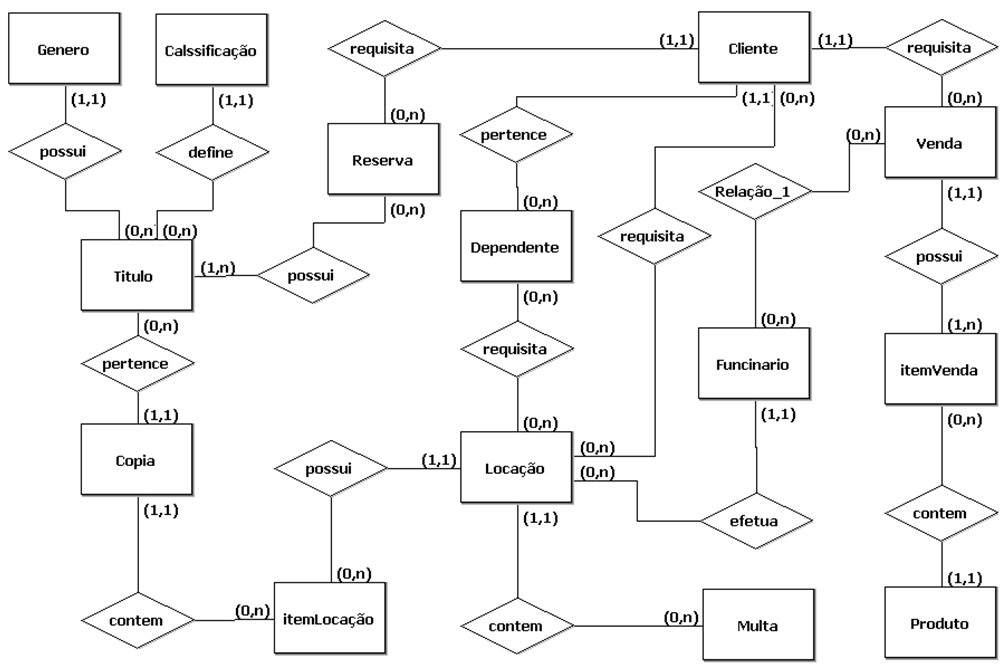
\includegraphics[width=1.0\linewidth]{figs/EntidadeRelacionamento.png}
%	\caption[Exemplo de Diagrama Entidade Relacionamento.]{Exemplo de Diagrama Entidade Relacionamento.}
%	\label{fig:EntidadeRelacionamento}
%\end{figure}


\subsection{Modelo Físico de Dados do Sistema}
%<Neste item deve ser realizada a criação física do banco de dados, ou seja, a criação de scripts.>

Os scripts abaixo representam a criação de tabelas do banco, já utilizando o modelo final definido. O código 3.1 apresenta o script de criação da tabela "docs", que contém os metadados do documento, já o código 3.2 apresenta o script de criação da tabela "docs\_fts", que armazena as páginas indexadas de cada documento.

\begin{lstlisting}[caption={Criação da tabela de documentos}, label={sql:criacao_docs}]
CREATE TABLE IF NOT EXISTS docs(
    id INTEGER PRIMARY KEY AUTOINCREMENT,
    nm_edicao TEXT UNIQUE NOT NULL,
    caminho TEXT NOT NULL,
    dt_edicao TEXT NOT NULL);
\end{lstlisting}
\noindent{\footnotesize Fonte: O autor (2026).}

A tabela "docs" apresentada no código 3.1 serve como um indice dos documentos que foram lidos e indexados, ela contém uma chave de id único para cada documento e seus dados básicos que são utilizados pelo frontend para listagem, além do link de acesso direto ao arquivo pdf do diário, armazenado na coluna "caminho".

\begin{lstlisting}[caption={Criação da tabela de indexação dos documentos}, label={sql:criacao_docs_fts}]
CREATE VIRTUAL TABLE IF NOT EXISTS docs_fts
USING fts5(doc_id, pagina, conteudo, tokenize = "unicode61 remove_diacritics 0");
\end{lstlisting}
\noindent{\footnotesize Fonte: O autor (2026).}

No caso do código 3.2, referente a criação da tabela de indexação de documentos, além das colunas definidas, também é passado para a função fts5 o parâmetro "tokenize" que permite escolher qual algoritmo será utilizado no processo de indexação textual na tabela, além de propriedades para o algoritmo. No caso deste trabalho foi utilizada a propriedade "remove\_diacritics 0" junto com o algoritmo unicode61, esta propriedade serve para que o algoritmo faça diferenciação de caracteres como "ç" e "c", caso a propriedade não seja definida o algoritmo faz o processo de "tokenização" destes caracteres de forma a considera-los como o mesmo caractere, o que pode refletir em resultados de busca indesejados.

\subsection{Dicionário de Dados do Sistema }

O banco de dados do sistema foi modelado para armazenar os metadados e o conteúdo dos documentos indexados, permitindo que as consultas textuais sejam feitas utilizando o mecanismo FTS5 do SQLite. Isso foi feito através de duas tabelas, a primeira é a tabela "docs" que armazena os dados dos documentos obtidos e funciona como principal entidade do sistema.

\begin{table}[h]
    \centering
    \caption{Tabela: docs}
    \label{tab:placeholder_label}
    \begin{tabularx}{\textwidth}{l l c X}
        \toprule
        Campo & Tipo & Chave & Descrição \\
        \midrule
        id & INTEGER & PK & Chave de identificação do documento indexado \\
        nm\_edicao & TEXT & & Campo que contém a edição (ex: 7389-A) do diário oficial  \\
        caminho & TEXT & & Campo que contém o link de acesso ao arquivo indexado\\
        dt\_edicao & TEXT & & Campo que contém a data do diário oficial em formato YYYY-MM-DD\\
        \bottomrule
    \end{tabularx}
\end{table}

A segunda é a tabela "docs\_fts", que é uma tabela criada utilizando o mecanismo FTS5 que serve como tabela de indexação do conteúdo dos documentos. É através dela que o recurso de busca textual do SQLite opera.

\begin{table}[h]
    \centering
    \caption{Tabela FTS5: docs\_fts}
    \label{tab:placeholder_label}
    \begin{tabularx}{\textwidth}{l l c X}
        \toprule
        Campo & Tipo armazenado & Chave & Descrição \\
        \midrule
        doc\_id & INTEGER & FK & Campo usado como chave estrangeira que aponta para a chave primaria da tabela docs \\
         pagina & INTEGER &  &  Campo que armazena o número da página indexada\\
         conteudo & TEXT &  & Campo que armazena o texto extraído da página \\
        \bottomrule
    \end{tabularx}
\end{table}

Todo o conteúdo dos documentos é separado por páginas durante a leitura do arquivo no módulo de scraping e cada página é armazenada separadamente na tabela. No SQLite, internamente todo conteúdo das tabelas criadas usando este mecanismo é tratado e otimizado como texto, por isso suas colunas não possuem tipo como foi possível visualizar anteriormente no código 3.2, os dados armazenados são parte de um índice invertido e são "tokenizados" para otimização de busca textual.

%<Neste item deve ser criado o dicionário de dados do banco de dados, com o obejtivo de documentar todas as tabelas, atributos, triggers e stored procedures.>

\section{Diagrama de Classe do Sistema}

A figura XX contém o diagrama de classes da API, que apresenta as classes de modelos de requisição, resposta e entidade do sistema.

\begin{figure}[htbp!]
    \centering
    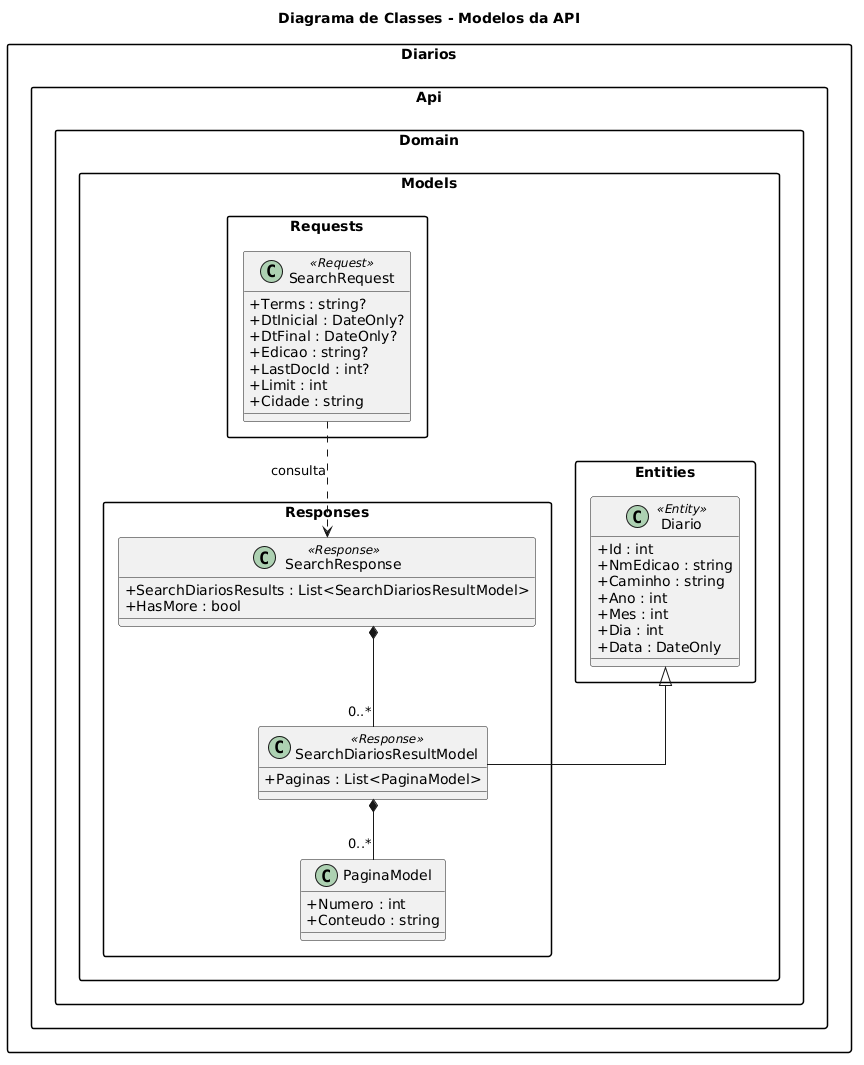
\includegraphics[width=0.8\linewidth]{figs//diagramas/DiagramaClassesApi.png}
    \caption{Diagrama de classes da API backend}
    \label{fig:placeholder}
\end{figure}

 O pacote de requests contém a classe "SearchRequest" que é o modelo de dados que a API espera receber para realizar a busca, nela está definido os campos de termos da busca, datas para a filtragem, edição, ultimo id de documento buscado, limite de documentos na resposta e cidade correspondente. No pacote de Responses a classe "SearchResponse" representa o modelo de retorno da busca, contendo uma lista de resultados encontrados, sendo estes os diários e o conteúdo das páginas que correspondem com os termos pesquisados para exibição de prévia no frontend.
%<Neste item deve ser apresentado o diagrama de classes completo do sistema. Fzer uma breve descição deste diagrama.>
%\begin{figure}[h]
%    \centering
%	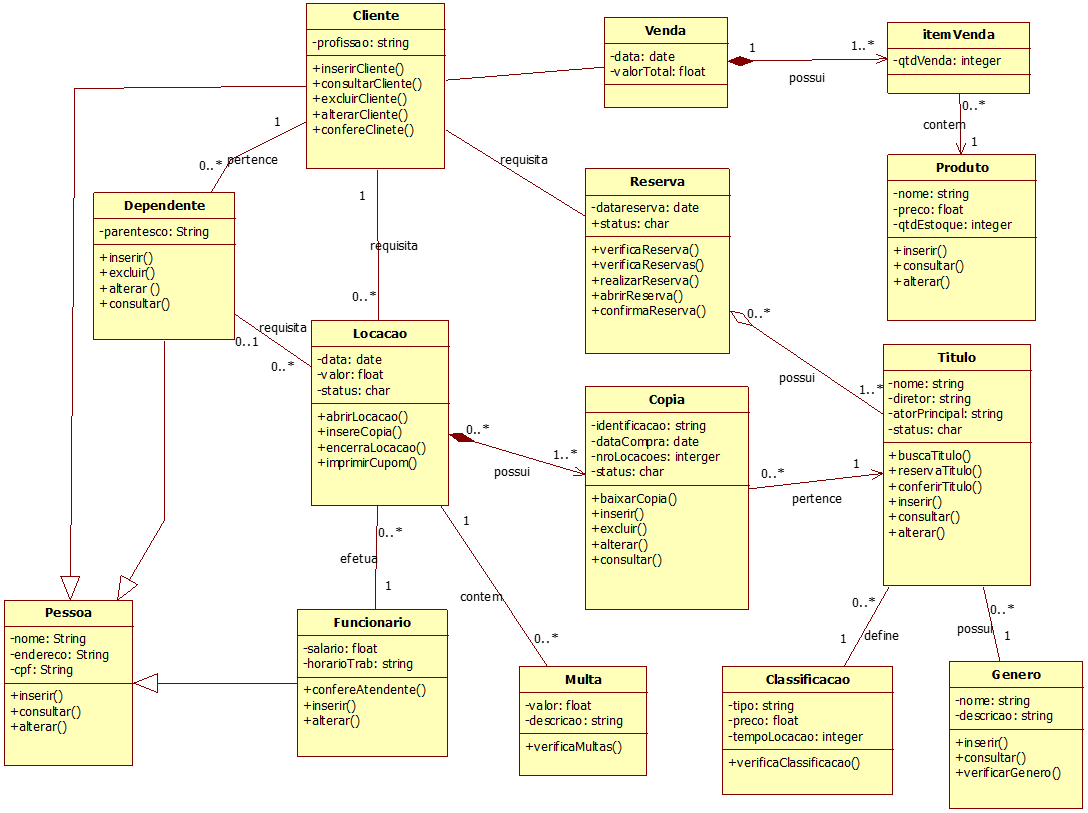
\includegraphics[width=1.0\linewidth]{figs/Classe.png}
%	\caption[Exemplo de Diagrama de Classe do Sistema.]{Exemplo de Diagrama de Classe do Sistema.}
%	\label{fig:DiagramaClasse}
%\end{figure}

\section{Diagramas de Atividades}

A figura XX demonstra o diagrama de fluxo de busca do sistema, que descreve o caminho percorrido desde a solicitação de busca pelo usuário até a exibição dos resultados e o diagrama de fluxo de coleta e indexação, que descreve o fluxo de obtenção dos documentos até o fim do processo de indexação.

\begin{figure}[h]
    \centering
    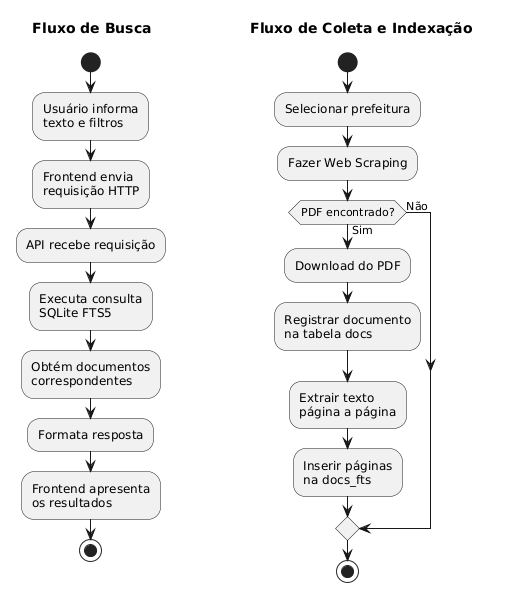
\includegraphics[width=0.6\linewidth]{figs//diagramas/FluxosJunto.png}
    \caption{Fluxos do sistema}
    \label{fig:placeholder}
\end{figure}

No fluxo de coleta e indexação, o software foi pensado para receber uma lista de parâmetros (flags) para dar início ao seu fluxo de execução, neste trabalho foram desenvolvidos dois fluxos, o principal, que faz a busca e indexação dos documentos presentes no site da prefeitura de Uberlândia, neste caso é informado ao programa as flags de download, cidade, ano e mês. A execução de busca no site da prefeitura, download e indexação dos documentos e seus metadados é realizada automaticamente. O segundo fluxo é o de indexação local, onde é possível utilizar arquivos salvos localmente para serem indexados, neste caso é necessário informar o documento, a cidade, URI de acesso ao documento, além do ano, mês e dia correspondente ao diário sendo indexado.

Já no fluxo de busca, o primeiro passo é a entrada dos termos de busca e filtros de data informados pelo usuário no frontend, os termos e filtros são então enviados para a API REST, que recebe a requisição e realiza a montagem das consultas que serão realizadas no banco de dados SQLite a partir de quais filtros e termos foram informados pelo usuário, a API então realiza a consulta monta uma resposta com a listagem dos documentos obtidos e suas páginas com conteúdo correspondente para pré visualização. Por fim o frontend recebe a resposta e exibe a listagem de documentos obtidos e uma prévia das páginas que contém o conteúdo textual pesquisado.

%<Neste item deve ser apresentado o diagrama de atividades, que representa o detalhamento de tarefas e o fluxo de uma atividade para outra de um sistema.  Nem todos os sistemas necessitam da elaboração do diagrama de atividades, pois nem todas as tarefas do sistema necessitam de um detalhamento. Com isso, deve-se analisar a real necessidade e no que este diagrama irá auxiliar na implementação do sistema, como: detalhamento de workflow, de métodos, entre outros.>

%\begin{figure}[h]
%    \centering
%	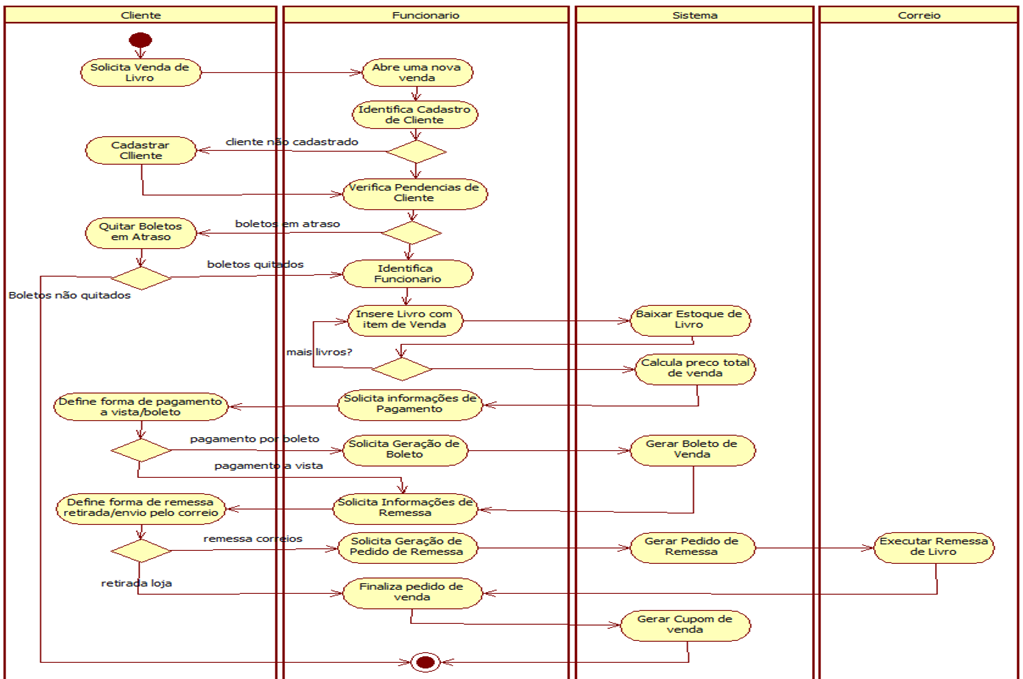
\includegraphics[width=1.0\linewidth]{figs/Atividades.png}
%	\caption[Exemplo de Diagrama de Atividades do Sistema.]{Exemplo de Diagrama de Atividades do Sistema.}
%	\label{fig:DiagramaAtividades}
%\end{figure}

\section{Diagrama de Implantação do Sistema}

Durante o desenvolvimento, foi utilizado um servidor VPS para a implantação e testes em um ambiente de execução mais próximo do real. A figura X representa o diagrama de implantação do sistema a partir desta implantação feita em desenvolvimento.

Um único servidor foi utilizado para a execução de todos os recursos desenvolvidos, no caso da API REST e do fronted web o gerenciamento é feito usando a ferramenta Docker Compose, usada para a definição da estrutura onde dois conteineres executam as aplicações separadamente, sendo um deles um container rodando o servidor web Nginx que opera para acesso ao frontend e também como proxy reverso para a API.

\begin{figure}[htp]
    \centering
    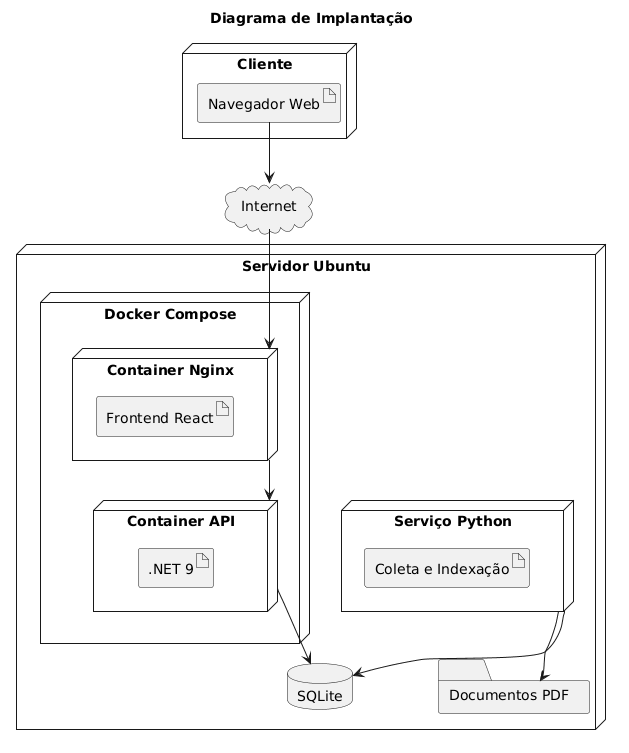
\includegraphics[width=0.6\linewidth]{figs//diagramas/DiagramaDeImplantacao.png}
    \caption{Diagrama de Implantação do Sistema}
    \label{fig:placeholder}
\end{figure}

 Já o serviço python de coleta e indexação opera diretamente no sistema operacional do servidor. A API tem acesso ao banco de dados que é compartilhado entre o sistema operacional do servidor e o container através de um volume compartilhado que é definido no arquivo YML de estrutura operado pelo Docker Compose, isto permite que o scraper e a API possam acessar a base de dados para realizar as operações de indexação e busca.

 No caso do servidor de desenvolvimento, o acesso através da internet aos serviços hospedados foi possível graças ao uso da ferramenta Cloudflare Tunnel, que possibilita a criação de um "tunnel" protegido entre o servidor e a rede da Cloudflare, facilitando a exposição do sistema na rede.

%<Neste item deve ser apresentado o diagrama de implantação que representa a arquitetura física de um sistema, mostrando como os componentes de software são alocados em hardware real. Ele visualiza a estrutura de execução de um sistema, incluindo nós (hardware e software) e o middleware que os conecta.>

%\begin{figure}[h]
%    \centering
%	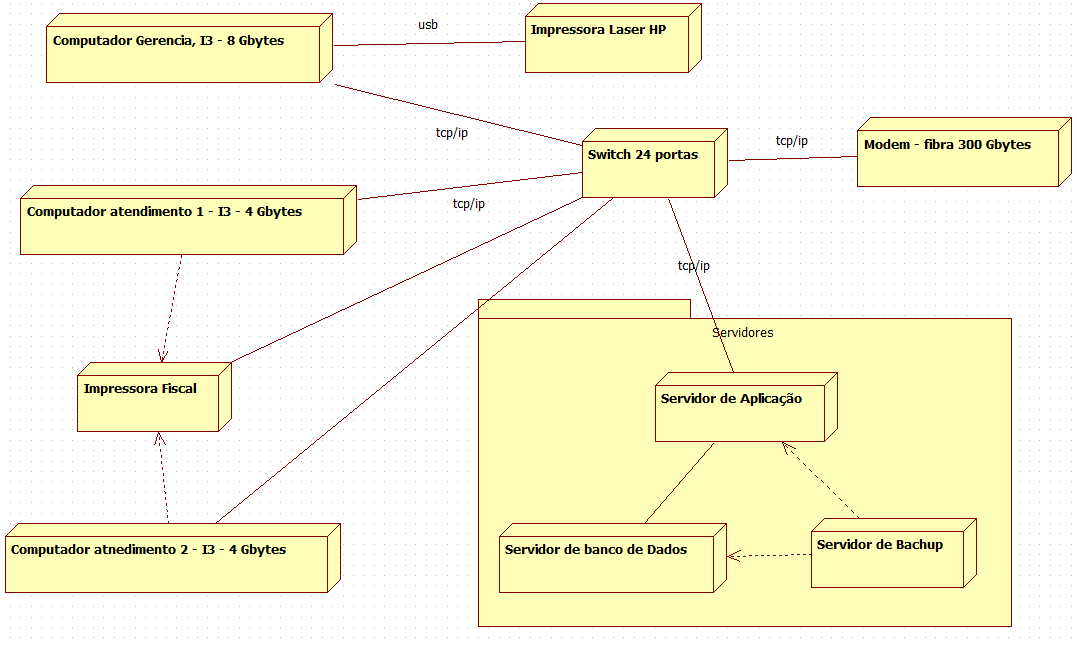
\includegraphics[width=1.0\linewidth]{figs/Implantação.png}
%	\caption[Exemplo de Diagrama de Implantação do Sistema.]{Exemplo de Diagrama de Implantação do Sistema.}
%	\label{fig:DiagramaImplantação}
%\end{figure}

\section{Considerações Sobre o Capítulo}
Este capítulo apresentou a análise e o projeto do sistema de recuperação de diários, contendo a modelagem de processos, estrutura de dados, componentes de software e a arquitetura de implantação utilizada. Os diagramas apresentados demonstram a interação entre os componentes do sistema e principais fluxos de execução, passando pela coleta de dados e indexação, até a realização de buscas e apresentação de resultados ao usuário.

A modelagem definiu a separação dos metadados dos documentos obtidos e o conteúdo textual extraído, utilizando o SQLite como ferramenta central utilizando do seu mecanismo de busca textual para a recuperação dos documentos.

Por fim, o diagrama de implantação apresenta a organização dos componentes em ambiente de execução, demonstrando a base de estrutura do sistema e como seus componentes são integrados. O capítulo seguinte aborda aspectos da implementação e funcionamento da solução desenvolvida.

%<Neste item deve ser apresentado as considerações sobre o capítulo, incluindo uma avaliação do que fio apresentado.>